\documentclass[10pt,preprint]{sigplanconf}

\usepackage[utf8]{inputenc}
% the following standard packages may be helpful, but are not required
%\usepackage{longtable}
\usepackage{mathtools}
\usepackage{multicol}
\usepackage{multirow}
\usepackage{booktabs}
\usepackage{courier}
\usepackage[scaled]{helvet}
\usepackage{url}
\usepackage{listings}
\usepackage{enumitem}
\usepackage{mdwlist} % tighter description environment (starred)
\usepackage[colorlinks=true,allcolors=blue,breaklinks,draft=false]{hyperref}
% known bug: http://tex.stackexchange.com/questions/1522/pdfendlink-ended-up-in-different-nesting-level-than-pdfstartlink
\newcommand{\doi}[1]{doi:~\href{http://dx.doi.org/#1}{\Hurl{#1}}}   % print a hyperlinked DOI

\usepackage{graphicx}
\usepackage{softdev}
\usepackage{amsmath}
\usepackage{mdwlist}
\usepackage{pifont}
\usepackage{xspace}

\newcommand{\kalibera}{Kalibera \& Jones\xspace}
\newcommand{\krun}{Krun\xspace}
\newcommand{\hypone}{H1\xspace}
\newcommand{\hyptwo}{H2\xspace}
\newcommand{\binarytrees}{\emph{binary trees}\xspace}
\newcommand{\richards}{\emph{Richards}\xspace}
\newcommand{\spectralnorm}{\emph{spectralnorm}\xspace}
\newcommand{\nbody}{\emph{n-body}\xspace}
\newcommand{\fasta}{\emph{fasta}\xspace}
\newcommand{\fannkuch}{\emph{fannkuch redux}\xspace}
\newcommand{\bencherthree}{4709K/Linux\xspace}
\newcommand{\bencherfive}{4790/Linux\xspace}
\newcommand{\benchersix}{4790/OpenBSD\xspace}
\newcommand{\bencherseven}{ARM\xspace}

\lstset{
    basicstyle=\tt\scriptsize,
    xleftmargin=2em,
    framexleftmargin=1.5em,
    numberstyle=\scriptsize\tt\color{gray},
    captionpos=b,
    escapeinside={{<!}{!>}},
}

\begin{document}

\title{Virtual Machine Warmup Blows Hot and Cold}
\authorinfo{Edd Barrett}
           {Software Development Team\\ Department of Informatics\\ King's College London}
           {http://eddbarrett.co.uk/}
\authorinfo{Carl Friedrich Bolz}
           {Software Development Team\\ Department of Informatics\\ King's College London}
           {http://cfbolz.de/}
\authorinfo{Sarah Mount}
           {Software Development Team\\ Department of Informatics\\ King's College London}
           {http://snim2.org/}
\authorinfo{Laurence Tratt}
           {Software Development Team\\ Department of Informatics\\ King's College London}
           {http://tratt.net/laurie/}

\maketitle

\noindent\textbf{Please note: this is a draft.}

\begin{abstract}
Warmup is magic.
\end{abstract}

\section{Introduction}
\label{sec:intro}

\laurie{we need a really simple graph in the intro, along the lines of the one
in the glowworm proposal. and not the current figure 1, whose caption is really
confusing!}

\laurie{since, at the moment, we don't say anything about how \emph{long} it
takes to warmup, i've not tried saying at all about that.}

Many modern languages are implemented as Virtual Machines (VMs) which use a
Just-In-Time (JIT) compiler to translate programs into machine code at run-time.
Since this compilation is not immediate, programs which are JIT compiled are
said to be subject to a \emph{warmup} phase. The common conception is that
during this phase, program execution is slow; then afterwards, execution is
fast. It is this ``traditional'' view on warmup that forms the basis for
benchmarking. Typically benchmarks are run repeatedly, and results collected
prior to warmup are discarded.

In this paper, we show that the following hypothesis does not hold:
\begin{description}
  \item[\hypone] Small, deterministic programs exhibit traditional warmup behaviour.
\end{description}

We present a carefully designed
experiment where a number of simple benchmarks are run on a variety of
VMs for a large number of iterations. We expected this to validate the above
hypothesis, allowing us to easily compare warmup across VMs. However, the
results are surprising: some benchmarks on some VMs run as per traditional
expectations; some never warmup at all, staying at their initial performance
levels indefinitely; and some `warmdown', getting slower over time. Even within
those benchmarks that appear to warmup in a traditional fashion, there are
various performance patterns that make presenting a simple performance number
difficult. Of the eight VMs we looked at,
none consistently warmed under the traditional model \edd{check this is true
when we have all the results}.

Our much wider ranging results suggest that, as a
field, we need to take a more nuanced view
of warmup. In general, we suggest it is better to think of most benchmarks as
generally converging on a \emph{steady state} of performance (be that faster or
slower than initial execution). When a benchmark does not converge on a steady
state, we suggest that it is impossible to give meaningful performance figures.
We believe our results are of interest to VM writers, but also to users of
those VMs. Authors may not have considered the different types of warmup
behaviour (or found benchmarks which trigger such behaviour), whereas users may
obtain a greater understanding of why their programs do not perform as well as
they had expected.

This paper's contributions are as follows:
\begin{enumerate*}
  \item \laurie{blah blah}
\end{enumerate*}

This paper's structure is as follows. \laurie{blah blah}


\section{Background}
\label{sec:warmup}

It has long been known that programs vary in performance from execution to
execution---in other words, that a single number is not sufficient to capture a
program's range of performance. The notion of confidence intervals is a good
first step towards capturing this notion for statically compiled
programs~\cite{fleming86notlying}. However, JIT compiled VMs offer an additional
complication: the performance of a program changes during execution. When a
program starts running on a JIT compiling VM, it is typically (slowly)
interpreted; once `hot' (i.e.~frequently executed) loops or methods are
identified, they are dynamically compiled into machine code; and subsequent
execution of those loops or methods uses (fast) machine code rather than the
(slow) interpreter. The period during which a JIT compiling VM hot portions of a
program are identified and compiled is referred to as \emph{warmup}; once all
such portions have been compiled, the program is said to be at \emph{peak
performance}.

\begin{figure}[h!]
\centering
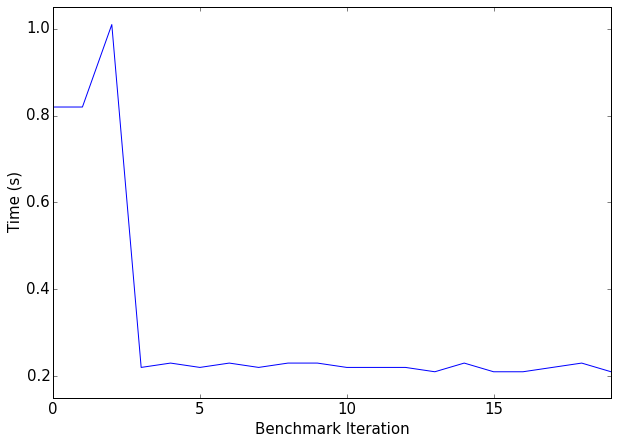
\includegraphics[width=.4\textwidth]{img/trad}
\caption{\laurie{the problem here is that we say `fictional', but the data looks vaguely real. we'd do better to make an obviously-not-real data figure, so that users can't misinterpret it. the glowworm proposal has something along these lines in it already} This (fictional) chart illustrates the commonly accepted understanding
of JIT performance. Early iterations of a benchmark perform poorly during the
warmup phase of the JIT. Once the JIT begins emitting native code (around
iteration 3) the latency of the benchmark is consistently small, with a small
amount of variation due to the operating system and execution environment.}
\label{fig:trad}
\end{figure}

Figure~\ref{fig:trad} shows the expected performance profile of an abstract
program under this model. Exactly how long warmup takes is highly dependent on
the program and the JIT compiler, but this basic assumption about the
performance model is shared by every JIT compiling VM.

Designing a benchmarking methodology which deals with the unusual nature of JIT
compiling VMs is hard. The most advanced VM benchmarking methodology we are
aware of is that of \kalibera~\cite{kalibera12quantifying,kalibera13rigorous}.
Benchmarks with multiple iterations must have their results inspected by a human
to manually determine when warmup has completed; all iterations before warmup
are removed, and the statistics proposed by \kalibera then applied (see
e.g.~\cite{barrett15approaches,grimmer15dynamically} for this scheme in use).
\kalibera note that some benchmarks have cyclical behaviour, for example where
pairs of iterations have low/high performance; users are required to
consistently pick an iteration and use that for statistical analysis. As we
shall see, identifying when warmup has completed is too tricky for humans to
reliably identify. It would also be far more satisfying to deal with cyclical
behaviour in a way that represents all parts, rather than a solitary part, of a
cycle.


\section{Methodology}
\label{sec:methodology}

To compare the warmup behaviour of different VMs, we created a carefully
designed experiment. The basic idea is simple: we take a number of
micro-benchmarks derived from the Computer Language Benchmarks Game (CLBG) and
run them in a loop of 2000 iterations on a number of VMs. We repeat this
process 10 times before analysing the resulting time series data. Our
experiment is designed to control as many potentially confounding variables as
is practical.

In this section we detail the set of benchmarks we use; the VMs under
investigation; our benchmark harness;
and the hardware we used. Readers may wish to note that we use two terms defined
by \cite{kalibera13rigorous}. \emph{Iterations} are in-process repetitions of a
benchmark, whereas \emph{executions} are repetitions using fresh processes.


\subsection{The CLBG micro-benchmarks}

We used the \binarytrees, \richards, \spectralnorm, \nbody, \fasta, and
\fannkuch microkbenchmarks from the CLBG, with implementations in C, Java,
Javascript, Python, Lua, PHP and Ruby. Readers can be forgiven for initial scepticism
about this set of micro-benchmarks. They are small and widely
used by VM authors as optimisation targets. In general they are more effectively
optimised by VMs than arbitrary programs; when used as a proxy for other types
of programs (e.g.~large programs), they tend to overstate the effectiveness of
VM optimisations. In our context, this weakness is in fact a strength: we need
small, deterministic, and widely examined programs so that we can test
hypothesis \hypone. Put another way, if we were to run arbitrary programs
and find unusual warmup behaviour, a VM author might reasonably counter that
``you have found the one program that exhibits unusual warmup behaviour''.

The CLBG micro-benchmarks often have multiple variants for a single language. We
used the variants from \cite{bolz14impact} as our starting point. We then
performed two separate checks / modifications on the variants to ensure their
suitability for our purposes.

The benchmarks were slightly modified for our purposes. Out of the box, the
CLBG the benchmarks are designed to be run once per process. Firstly, we
modified each benchmark so that our harness can run them repeatedly in-process.
An important aspect of this step involves locating and removing control flow
non-determinism. By this we mean that benchmarks should take precisely the same
path through the Control Flow Graph (CFG) on each iteration. Although this
should remove some sources of variation, note that it does not preclude the VM
having other types of non-determinism (e.g.~objects in memory may be allocated
or collected in a non-deterministic fashion). We identified CFG non-determinism
by instrumenting CFG choice points with \texttt{print} statements and compared
the output across multiple runs (\edd{how many}). This showed that the \fasta
benchmark was non-deterministic in all language variants, as it used a random
seed which was
initialised only on the initial load of the program; thus each iteration of the
program acquired different random numbers, causing different paths to be taken
through the CFG. We removed this non-determinism by putting the seed
initialisation in the main loop of the benchmark. Bearing in mind surprising
results such as the importance of link order \cite{mytkowicz09surprising}, we
then recompiled all the VMs and ran them on a different machine to see if any
compile-time constants affected determinism. \laurie{CF: please check to see if
the remainder of this paragraph is right} This showed that the Java class loader
initialises classes in a non-deterministic order, which affected the way that
some parts of Java benchmarks were executed in \laurie{as I wrote that, I became
aware that I don't really understand why this source of non-determinism crept
into our benchmarks. Was it inside the main loop? If so, how?} \laurie{i now
think the problem is that classes are loaded lazily as they are used, though i
admit i'm not sure how our nondeterminism checks spotted this}.

Second, to avoid measuring I/O, we removed all writing to standard output from
the benchmarks. By doing so however, we may unintentionally cause computations
to be removed. Advanced compilers and VMs, may be able to prove that the
results of a benchmark are not used, and may therefore optimise away large
parts of the benchmark. To avoid this, we introduced checksums into the
benchmarks. The checksums are simply a value whose value is tightly coupled
with the computational work of the benchmarks. After each iteration the value
of the checksum is checked against an expected value. If the values don't
match, an error is printed and the benchmark is terminated. For properly
implemented benchmarks, checksum errors do not occur, but since the condition
under which the error is printed is interwoven into benchmark computations,we
make it very difficult for a compiler or VM to optimise away large chunks of
the benchmark. As a bonus, the checksums serve to check that each of the
different language implementation do roughly the same work, but also they do a
limited form of CFG determinism checking.

We ran 10 executions of each benchmark, each execution comprising of 2000
iterations. For the avoidance of doubt, and in
contrast to some other experiments we are aware of \laurie{can we cite?}, we did
\emph{not} force a collection after each iteration, as a VMs GC is an important
factor in warmup.


\subsection{VMs under investigation}

We ran the benchmarks on a collection of modern programming language VMs,
as well as GCC as a baseline:
\begin{description*}
\item[GCC] On Linux systems, version 4.9.2 from Debian packages; on OpenBSD the base version 4.2.1.
\item[CPython 2.7.10] The reference Python implementation.
\item[Graal \#9dafd1dc5ff9] Oracle's next-gen VM targeting Java.
\item[HHVM 3.7.1] Facebook's PHP JIT.
\item[JRuby/Truffle \#7f4cd59cdd1c8] A Ruby interpreter using Graal for dynamic compilation.
\item[Oracle Java 8u45b14] Oracle's Hotspot VM for Java.
\item[LuaJIT 2.0.4] A tracing JIT for Lua.
\item[PyPy 4.0.0] A meta-tracing VM for Python-2.7.
\item[V8 4.8.271.9] Google's JIT for Javascript.
\end{description*}

All VMs were built with the same version of GCC/G++ as used for the baseline C
benchmarks, apart from where OpenBSD's GCC-4.2.1 was too old (PyPy, Oracle Java
and V8). In these cases, GCC-4.9.3 (from OpenBSD packages) was used.\footnote{In
future versions of this paper, we plan to use the same C compiler version
across the board.} We ran benchmarks on Debian Linux (the main source of
results in this paper) and
OpenBSD. All VMs were run on Linux; neither HHVM nor JRuby/Truffle has yet been
ported to OpenBSD, and we thus have no data for those VMs on OpenBSD.


\subsection{\krun}

Although running benchmarks is a conceptually easy, in practise it is a fiddly task:
VMs need to be built carefully; benchmarks need to be run in a consistent
environment; and errors need to be detected and reported to the user. We first created
a build script which automates the building of all the VMs in our experiment, allowing
us to predictably build VMs on multiple machines. We then created \krun: an
benchmark harness which automates benchmarking. \krun aims to be a generic tool
with utility beyond this paper, though we do not explore that further.

The basic architecture of \krun is as follows. A top-level supervisor script
\texttt{krun.py} is the starting point for an experiment. This reads in a
configuration file which describes to \krun which benchmarks are to be run, and
which VMs they will run under, as well as the number of in-process iterations
and executions to run. \krun then builds a work queue and begins running
executions of benchmarks. For each execution, \krun forks an \emph{iterations
runner}, whose role is to collect a series of in-process iteration times. Since
the timings must be collected in-process, there are many iterations runners:
one implemented in each language involved in the experiment. \krun passes
arguments to the iterations runner which specify which benchmark to run, a
number of iterations, and a \emph{benchmark parameter} which is used to
calibrate the length of an iteration. The iterations runner dynamically imports
the correct benchmark and times calls to a benchmark function in a loop. Once
the desired number of iterations have been collected, the iterations runner
returns a list of iteration times (the times for one execution) back to \krun.
The results are accumulated on-disk in a JSON file. \krun can be configured to
email the user should any benchmarks crash, or generate unexpected results.

Aside from being a simple benchmarking harness, \krun also aims to control as
many confounding variables as is practically possible. Some of the factors that
\krun controls are generic, whereas others are platform-specific. In the
following subsections we discuss these.

\subsubsection{Platform Independent Controls}

First, \krun does its best to maintain a consistent system temperature and to
prevent machines from overheating, which may lead to CPUs being throttled (and
thus distorting performance results). Initial temperature readings are taken
prior to the first benchmark execution, then prior to subsequent executions
\krun waits for the CPU to cool to within 10\%{} of the starting temperatures.
If the system fails to cool down within 10 minutes, \krun terminates with an
error.

Second, \krun has \emph{reboot mode}, which we use for our experiments. Before
each benchmark execution (including the first), \krun reboots the system and
re-invokes itself when the system comes back up. After a 3 minute wait (to
allow the system to fully come up), \krun then resumes benchmarking. This means
that the system is in a fresh "known" state prior to each execution,
essentially ensuring that later benchmark executions do not have an unfair
advantage due to, (for example) fewer cache misses. Note that this mode does
not preclude the use of the temperature control feature, as the starting
temperatures are stored to disk and read in prior to each execution.

Other platform-independent controls include the following. \krun imposes a
consistent heap and stack \texttt{ulimit} for each VM (we used a 2GiB heap and
a 8MB stack).\footnote{Note that some systems, e.g. Linux, do not honour
ulimits.} It also notifies the user should the system \texttt{dmesg} buffer
change. This feature was implemented after we found performance critical
messages in the \texttt{dmesg} buffer of one of our machines (this machine was
not used for the proper experiment, and has since been decommissioned).

\subsubsection{Platform Dependent Controls}

\edd{xxx}

\subsection{Machines used}

We used three machines and two operating systems:
\begin{description*}
  \item[\bencherthree] A quad-core i7-4790K 4GHz machine running Debian 8.
  \item[\bencherfive] A quad-core i7-4790 3.6GHz machine running Debian 8.
  \item[\benchersix] Identical hardware to \bencherfive, but running OpenBSD 5.7.
\end{description*}
These machines allow us to investigate the effects of moderately different
hardware (\bencherthree and \bencherfive have identical operating system and
package installation) as well as moderately different operating systems
(\bencherfive and \benchersix have identical hardware, but different Unix
variants). We started with the following hypothesis:
\begin{description}
  \item[\hyptwo] Moderately different hardware and operating systems have little effect on warmup patterns.
\end{description}
We deliberately use the word `moderately', since significant changes of hardware
(e.g.~ARM) or operating system (e.g.~Windows) implies significantly different
parts of the VMs will be used (e.g.~different machine code backends may be of
differing levels of maturity).

On Intel machines, we disabled turbo boost and hyper-threading in the BIOS. Turbo boost is a
feature which allows CPUs to temporarily run in an extremely high-performance
mode; this eventually causes the CPU to exceed its safe thermal limit, and
performance is then reduced to a lower limit. Turbo boost can thus cause long-running processes to
appear to suddenly slow down. Hyper-threading gives the illusion that a single
physical core is in fact more than one core, allowing more programs to
run semi-simultaneously. However, hyper-threading causes programs to interfere
with each others in complex ways, introducing considerable noise. It is of
no real benefit in our situation, where we do not even make use all of the
physical cores in our benchmarking machines.


\subsubsection{Linux}

On Linux, \krun controls several additional factors.

First, it attempts to fix the CPU frequency to the highest
possible `recommended' value (i.e.~below the overclocking range). This is achieved by disabling Intel
p-states support in the kernel and setting the CPU governor to \texttt{performance}
mode.~\footnote{This is our best attempt at obtaining a constant CPU clock
speed. The Linux kernel documentation states that ``the idea that frequency can
be set to a single frequency is fiction for Intel Core
processors''~\cite{XXX}.}

Second, it runs benchmarks on a single CPU core, reducing the cost of processes
being forcibly moved to different cores. This is achieved through Linux's
\texttt{isolcpus} feature. \laurie{this sentence scares me. i thought it would
mean that kernel threads wouldn't run on the core!} This means that benchmarks
share a CPU only with kernel threads. In theory a core can be fully isolated,
however the Linux tool to enable this is currently broken
\url{https://bugs.debian.org/cgi-bin/bugreport.cgi?bug=796893}.

Third, \krun minimises the effects of the Linux kernel profiler \laurie{can we
be clearer about what this thing is actually doing?}. We found this to introduce
substantial noise into benchmarks, since it dynamically adjusts (lowers
\laurie{can it only ever lower? can it raise?}) its sample rate if it is found
to spend too much CPU time. While this feature cannot be entirely disabled on
x86-64, \krun reduces its frequency to once per second, minimising noise.


\subsubsection{OpenBSD}

\laurie{sysctl to 100 and \texttt{apm -H} but p-states...?}


\subsection{Other stuff}

\edd{data layout (e.g. ASLR, don't re-run in separate sessions)}
\edd{quartile regression}


\section{Results}
\label{sec:Results}

After running all benchmarks as described we analysed the benchmarks in a
two-step process. In the first step we visually inspected the run sequence
graphs of all the benchmark executions, per benchmark and virtual machine. In
doing so we noted whether the virtual machine followed the expected warmup
behaviour for this benchmark as described in Section~\ref{sec:warmup}. This was
the case of \cfbolz{add numbers} X out of Y benchmarks. In a second step we
identified groups of ``anomalies'', i.e. repeating ways of how benchmark
executions deviated from the expected warmup behaviour. In the following we will
present the run-sequence diagrams of benchmarks that have expected warmup
behaviour, as well descriptions and examples for all the anomalies.

\cfbolz{need some examples of nice benchs}
\cfbolz{we need a table which does all the categorizations, and examples}

\cfbolz{observations 2x2: widely varying performance on the same machine, late
phase change not always there, another case: bimodality, slowdowns are
sometimes speedups, different repeating shapes across machines}

\cfbolz{safety checks: are outliers deterministic across different processes?
is the behaviour generally the same looking? do some checks on other OS,
machine architecture, frequency scaling independent}


\sarah{Warm-up takes longer than expected, by comparison with the idealised JIT
described in Section 2.}


\subsection{Outliers}
\label{sub:outliers}

Outliers are iterations of a benchmark that take significantly longer than the
other iterations, even taking the randomness of the benchmark iterations into
account.

Figure~\ref{fig:examples:outliers1} shows one such example, which includes an
outlier around iteration $900$ that runs more than $0.5s$ slower than the
measurements either side of it.

\begin{figure}[h!]
\centering
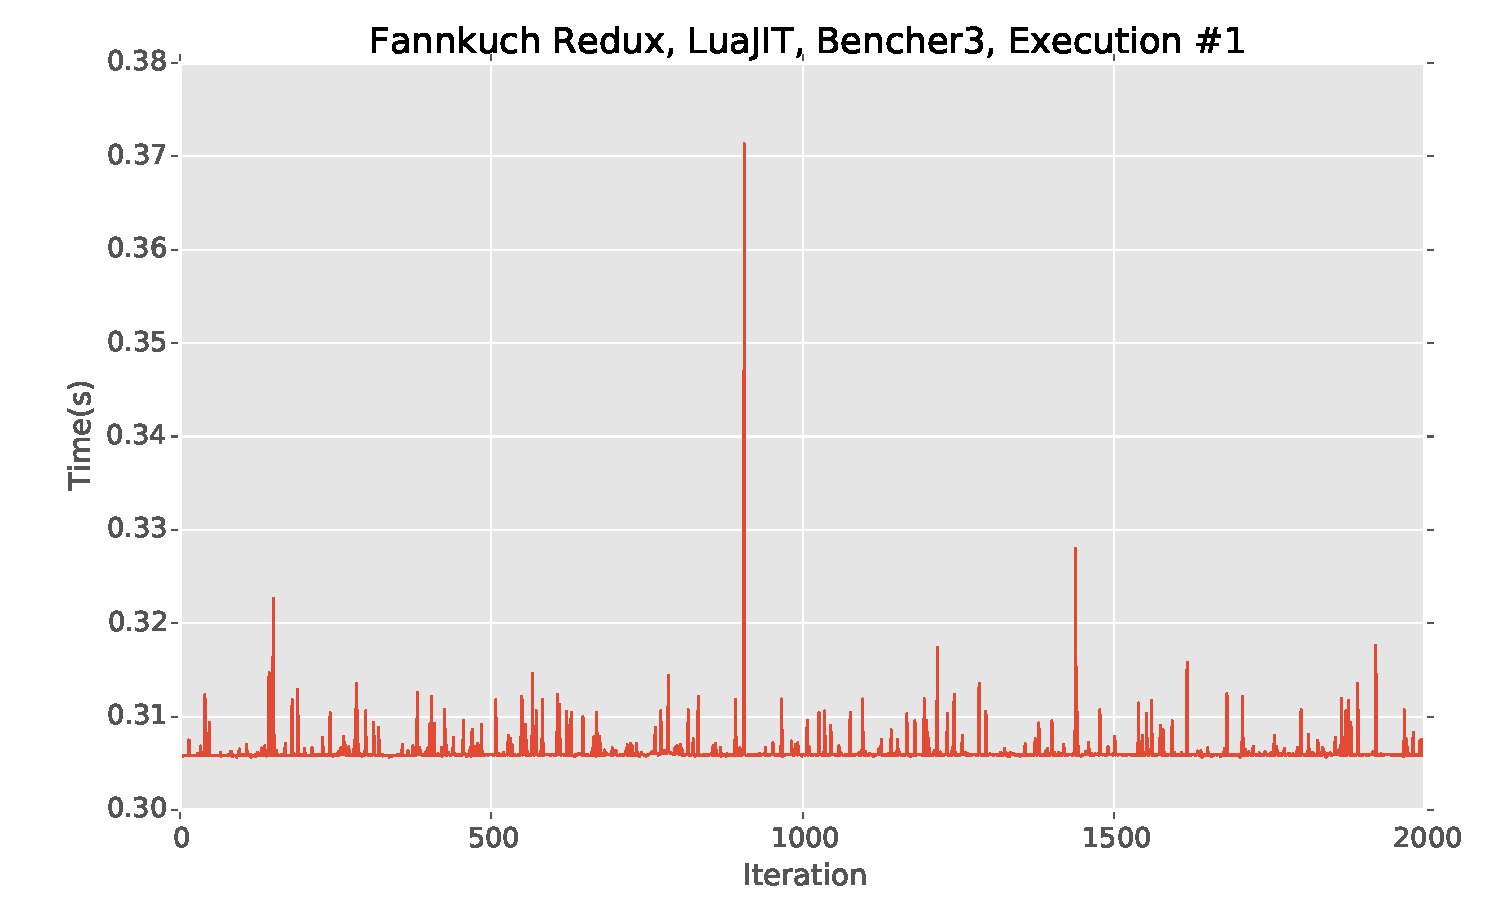
\includegraphics[width=.46\textwidth]{examples/outliers1}
\caption{Example of a benchmark with outliers.}
\label{fig:examples:outliers1}
\end{figure}


\subsection{Slowdowns}
\label{sub:slowdowns}

\sarah{This is one area were the sliding-window average might be useful (i.e. in detecting a slow-down).
One possible way forward would be to find a technique for performing hypothesis testing on time-series data, then running tests to determine whether the sliding-mean in one part of the chart is significantly different to the sliding-mean in an earlier phase of the execution.
This technique would also help to determine precisely when the warm-up phase is over and the JIT has kicked in.}

A few benchmarks exhibit slow downs, where the first few iterations of a
benchmarks are faster than the eventual mean after ``warm up''.

Figure~\ref{fig:examples:slowdown1} shows one such example.

\begin{figure}[h!]
\centering
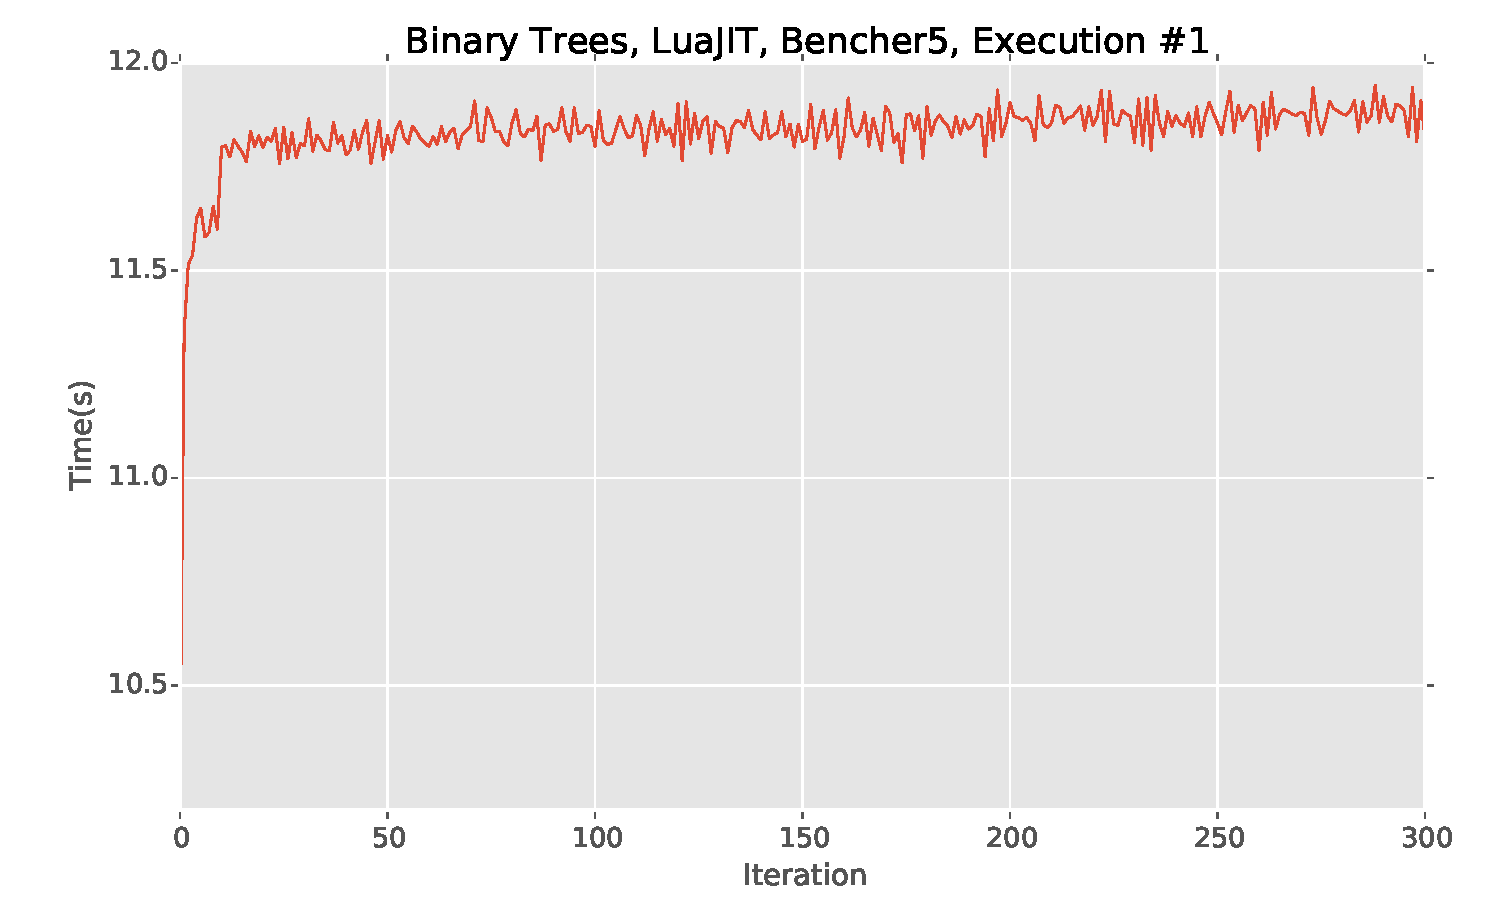
\includegraphics[width=.46\textwidth]{examples/slowdown1}
\caption{Example of a benchmark with a slowdown.}
\label{fig:examples:slowdown1}
\end{figure}



\subsection{Cyclic Behaviour}
\label{sub:cyclic}

Cyclic behaviour occurs in a number of benchmarks, which is a pattern of $n$
iterations that have similar timing results and keeps repeating across the
benchmark runs.

Figure~\ref{fig:examples:cycles1} shows one such example.

\begin{figure}[h!]
\centering
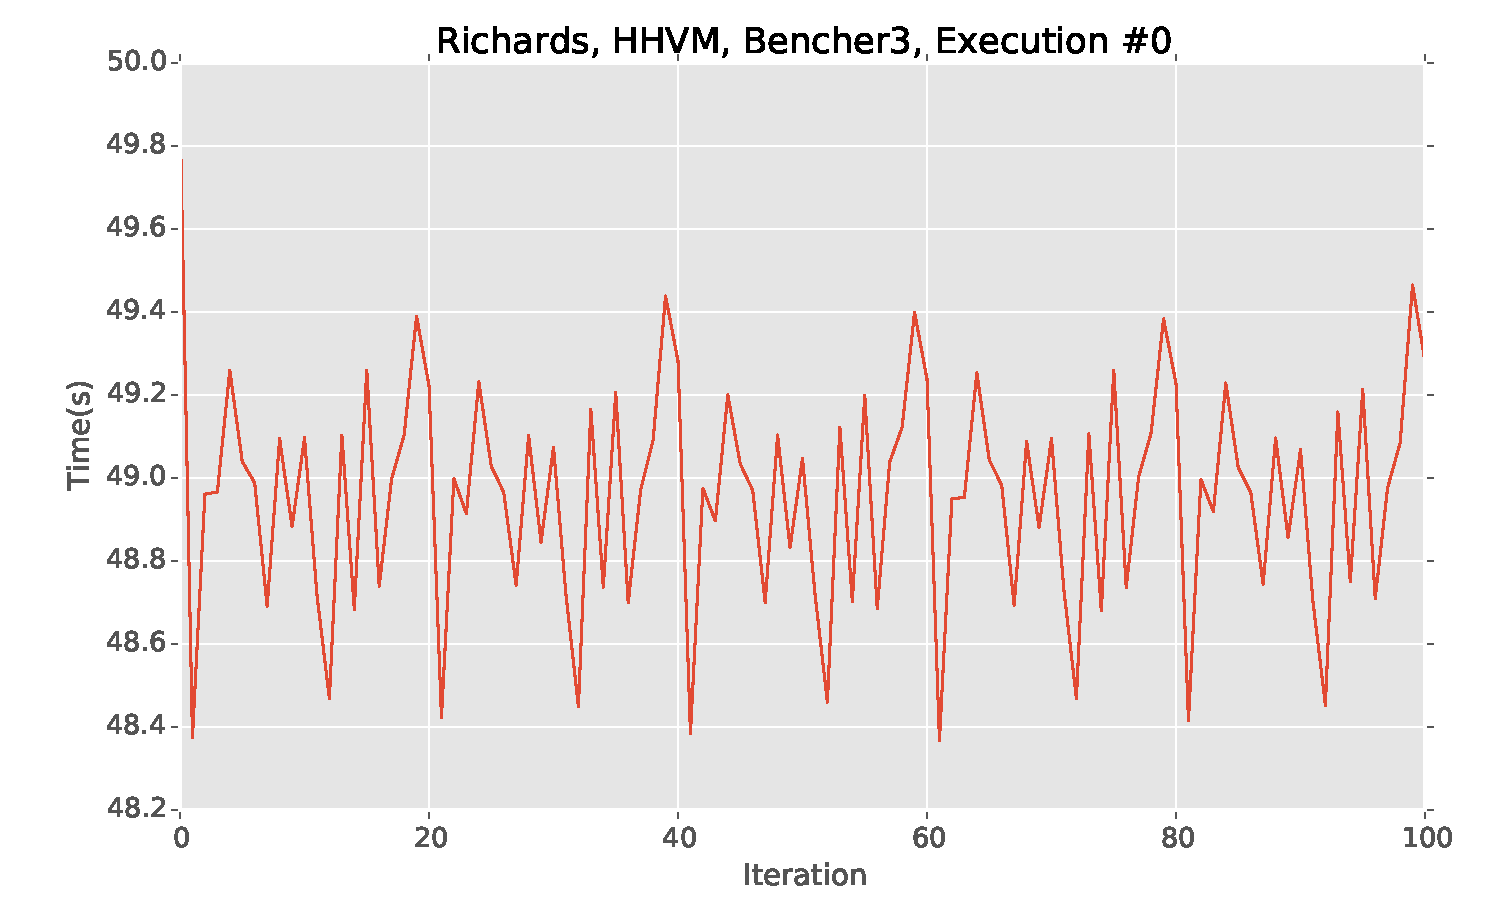
\includegraphics[width=.46\textwidth]{examples/cycles1}
\caption{Example of a benchmark with cycles.}
\label{fig:examples:cycles1}
\end{figure}


\subsection{Late Phase Changes}
\label{sub:phase}

Late phase changes occur in benchmarks where after many iterations the benchmark
changes behaviour, either by getting slower or faster, or by producing a
different pattern of randomness.

Figure~\ref{fig:examples:late1} shows one such example.

\begin{figure}[h!]
\centering
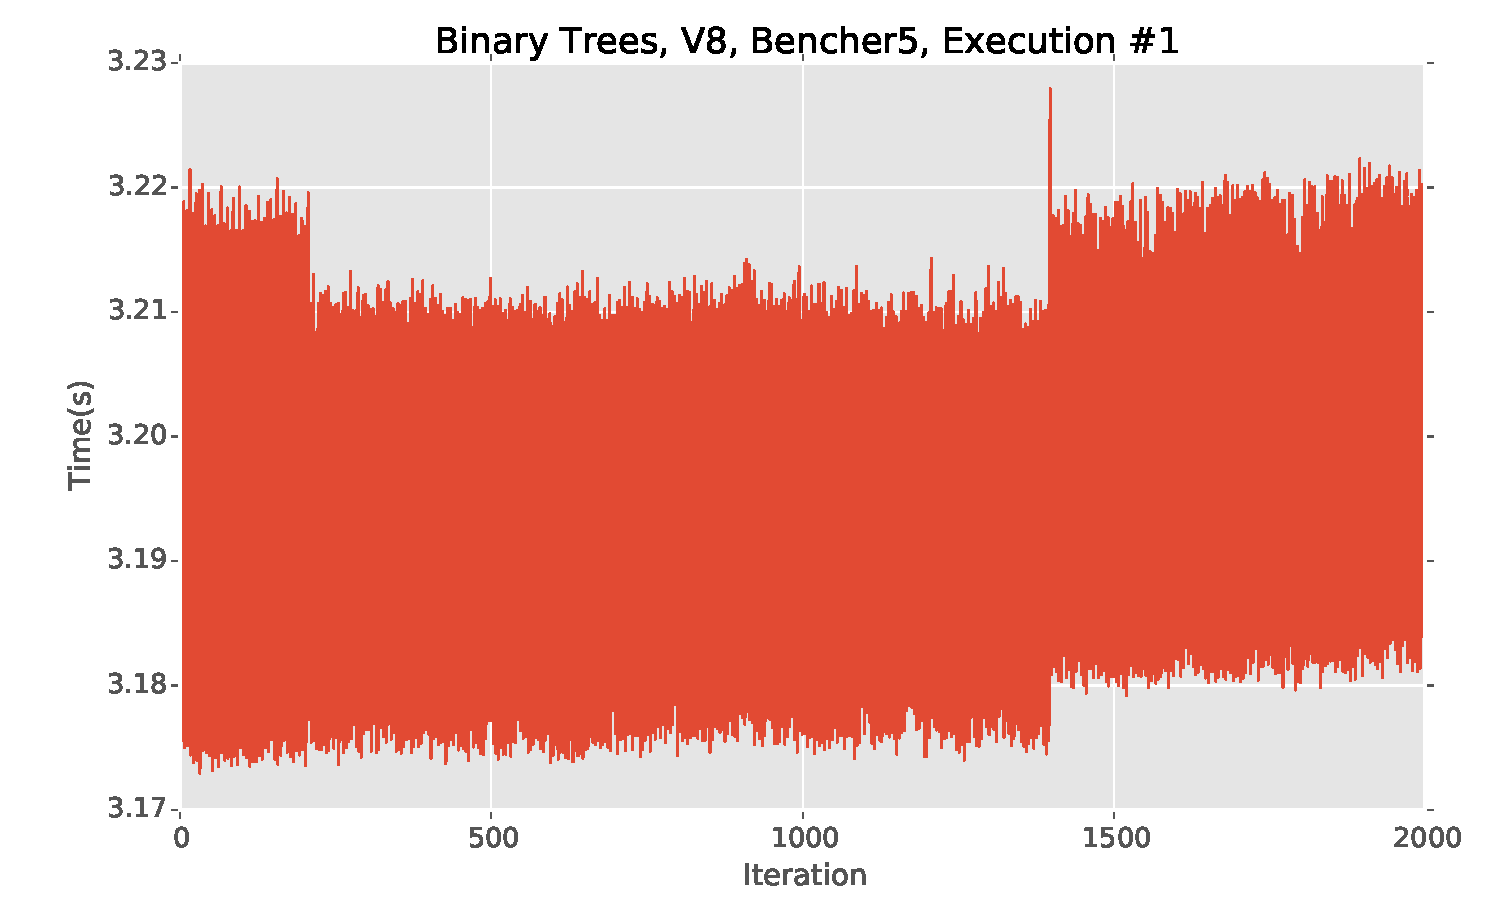
\includegraphics[width=.46\textwidth]{examples/late1}
\caption{Example of a benchmark with late phase changes.}
\label{fig:examples:late1}
\end{figure}

\subsection{Inconsistent Effects}
\label{sub:inconsistent}

\edd{Many of the effects we saw are consistently weird. Some are not. What
do we think of this as a section?}
\sarah{Sounds good, what about a section on unexpectedly long warmup?}

Figure~\ref{fig:examples:consistent_weirdness1} shows a case where
unexpected behaviours are consistent between machines and executions.
Figure~\label{fig:examples:inconsistent_weirdness1} shows an example where
effects differ between both machines and executions.

\begin{figure*}[h!]
\centering
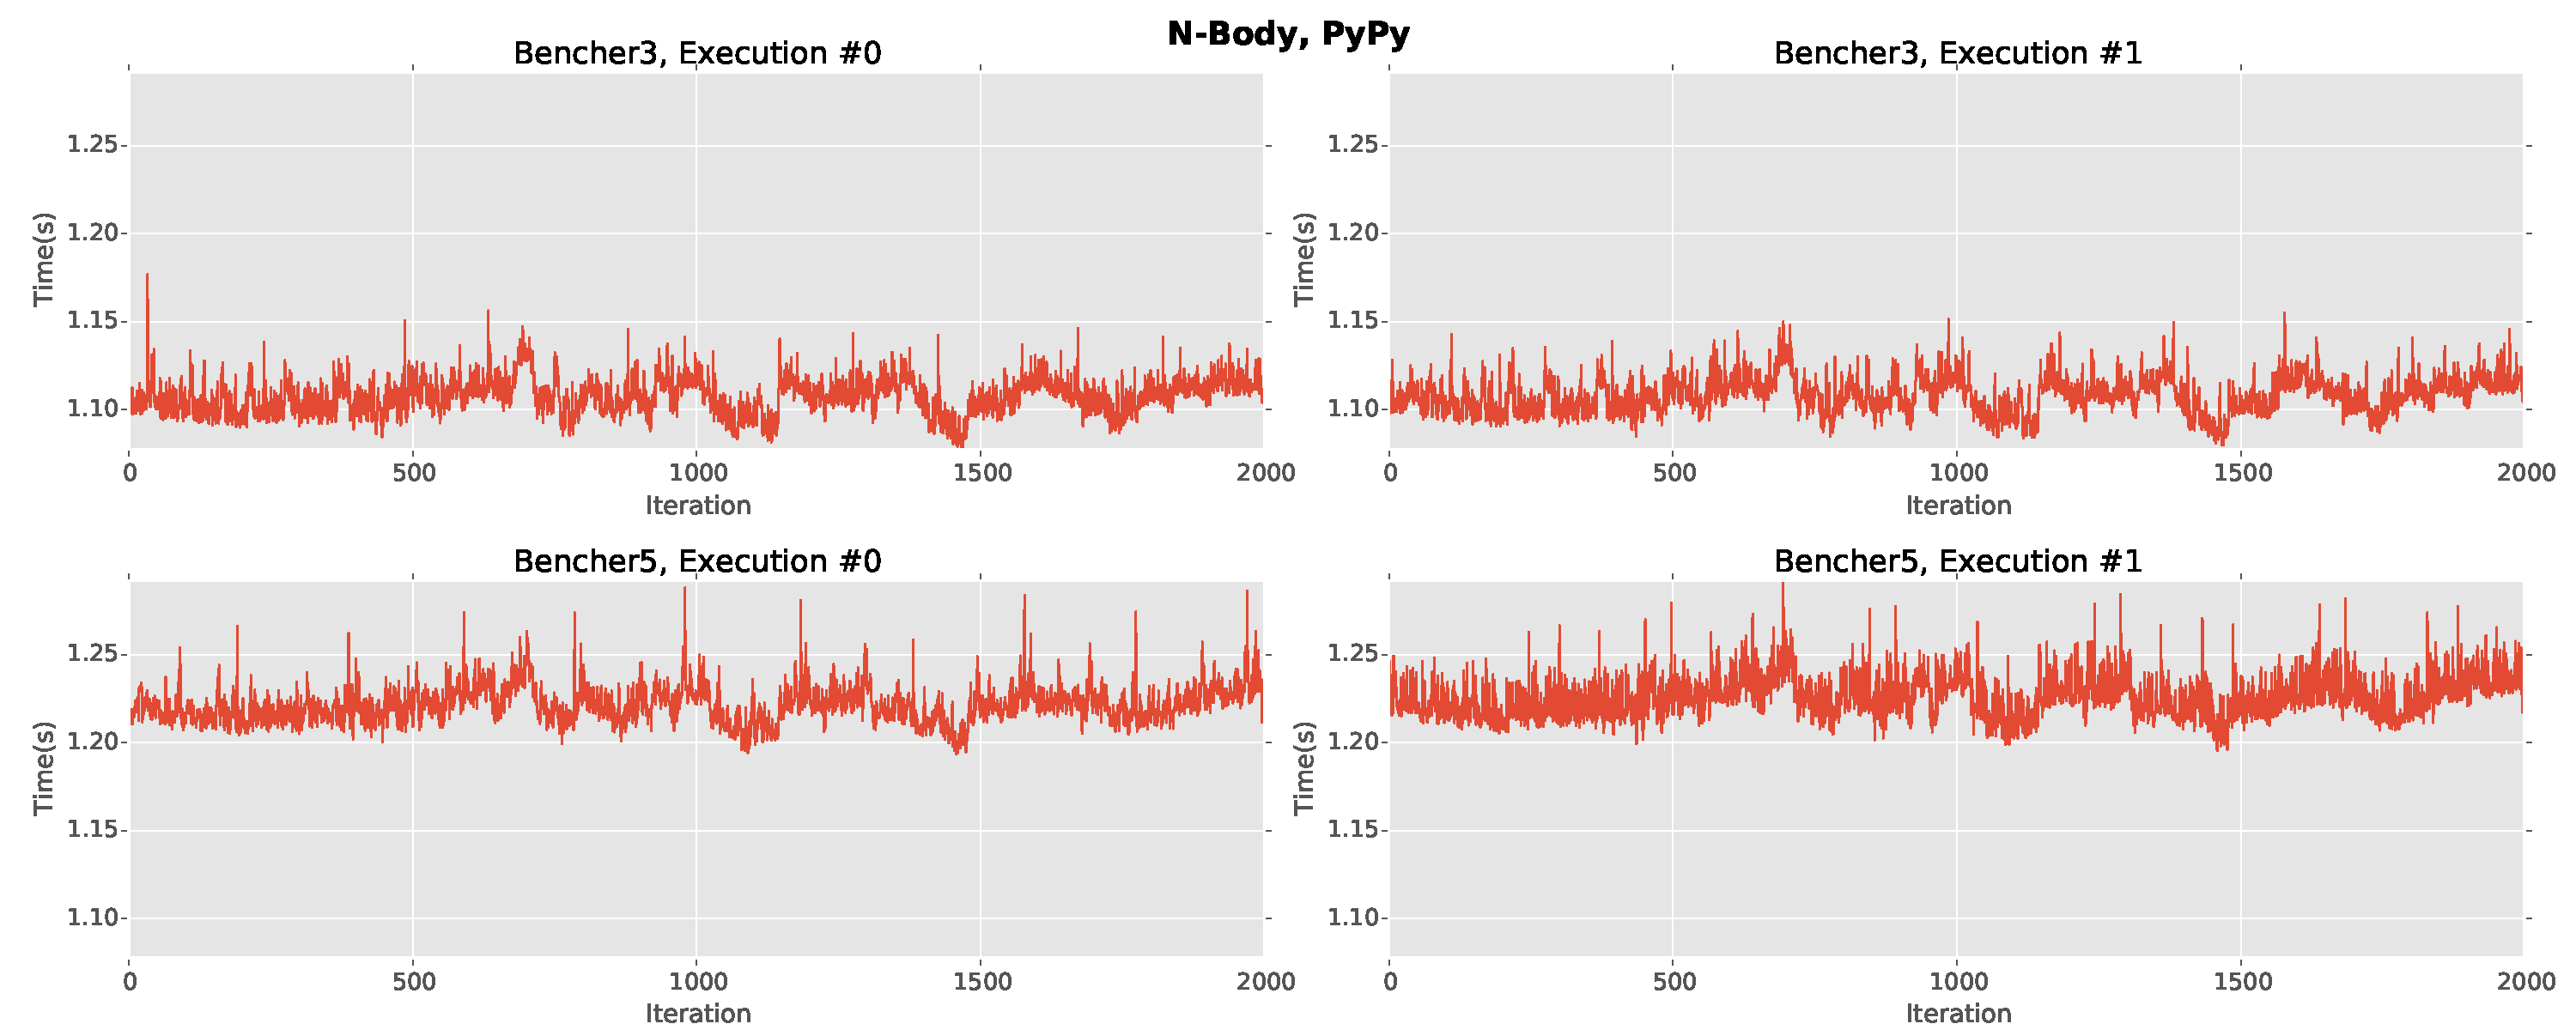
\includegraphics[width=\textwidth]{examples/consistent_weirdness1}
\caption{Example of a benchmark whose effects are consistent between machines and executions.}
\label{fig:examples:consistent_weirdness1}
\end{figure*}

\begin{figure*}[h!]
\centering
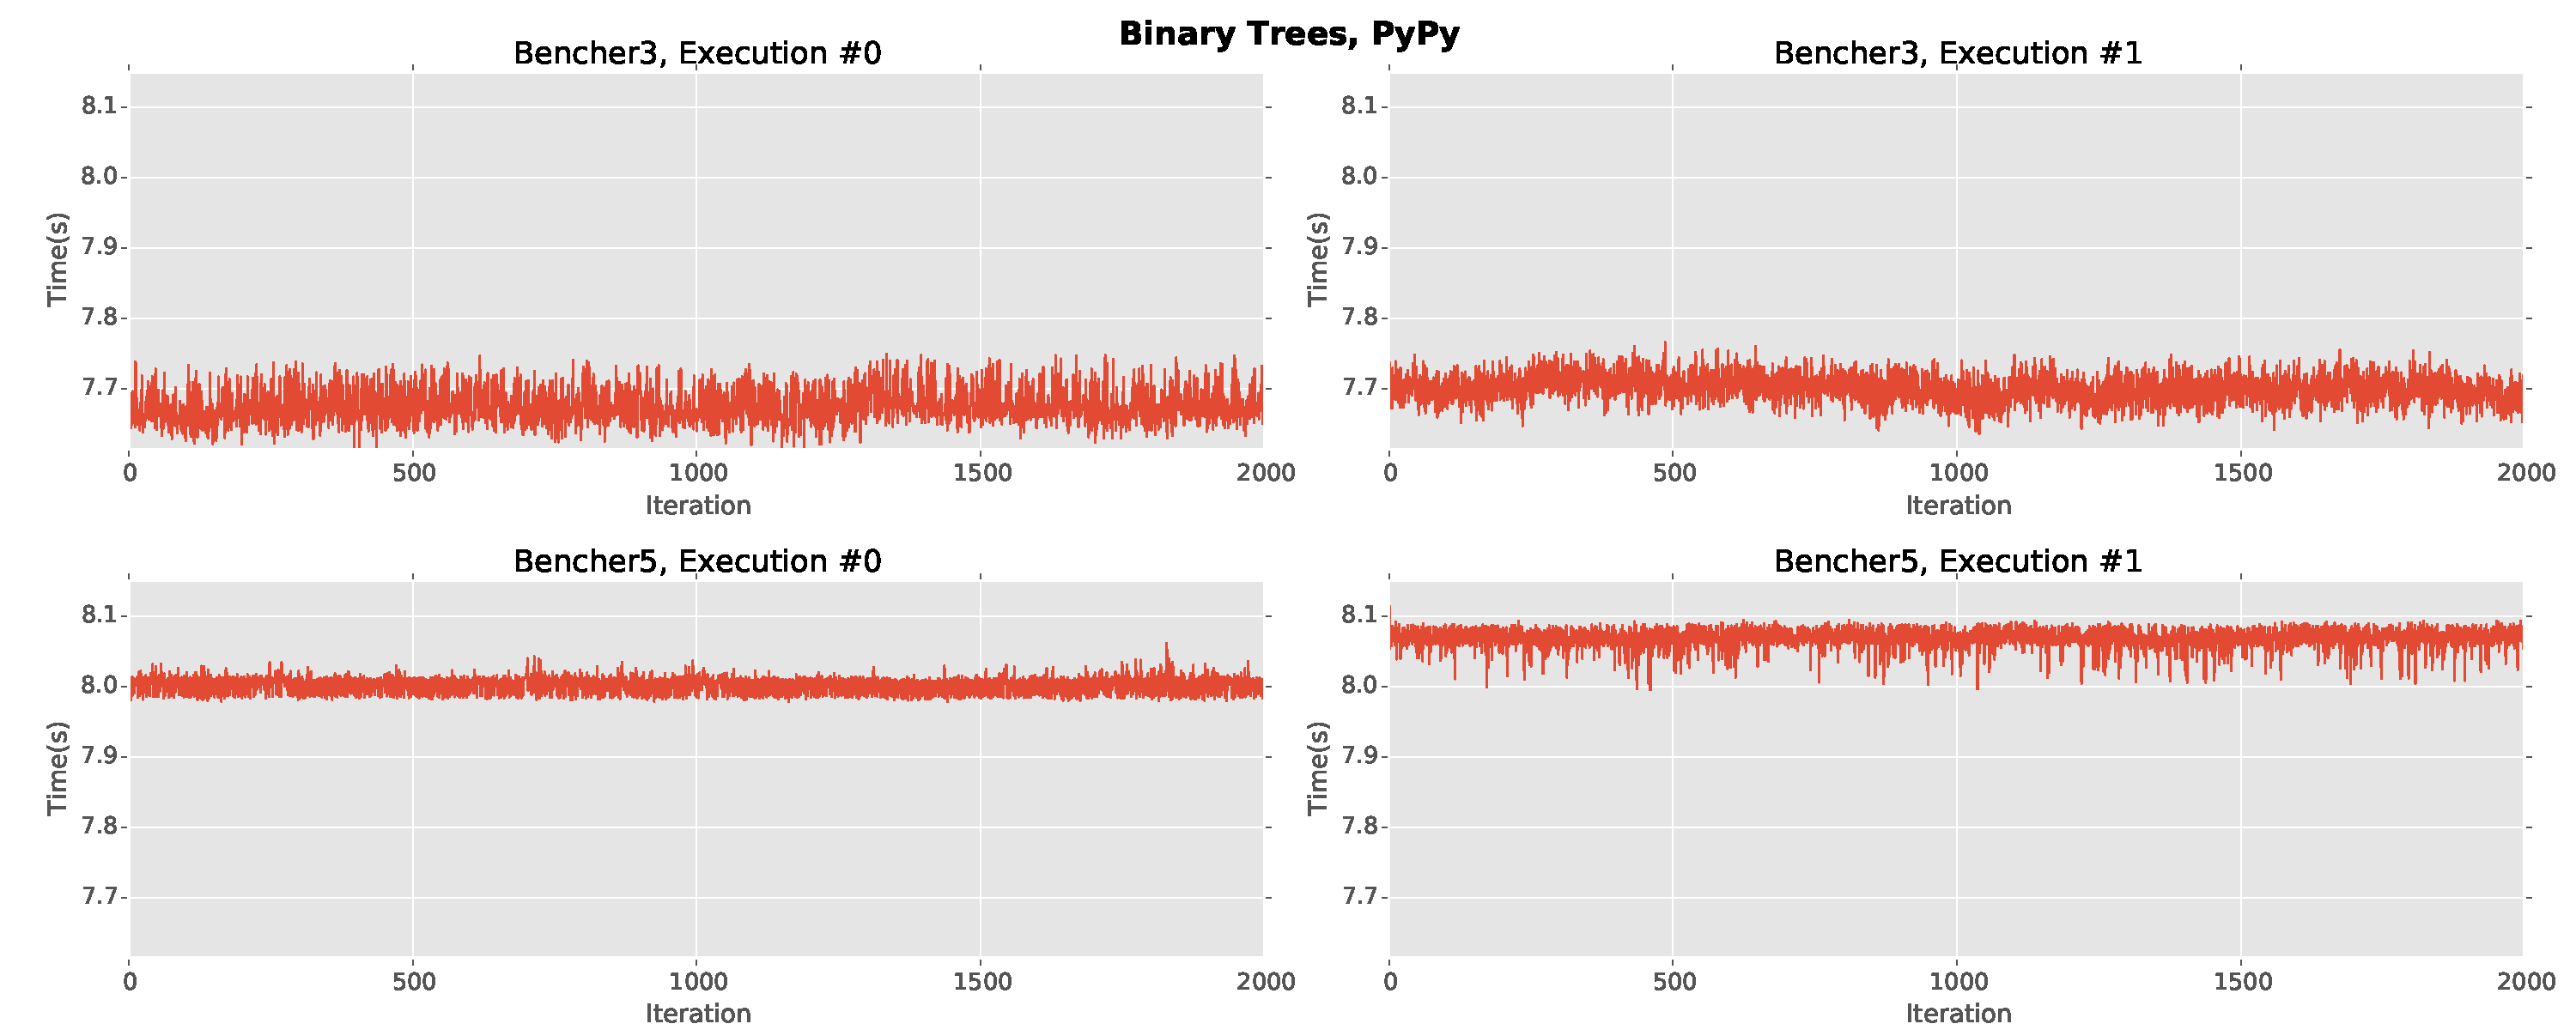
\includegraphics[width=\textwidth]{examples/inconsistent_weirdness1}
\caption{Example of a benchmark whose effects are inconsistent between machines and executions.}
\label{fig:examples:inconsistent_weirdness1}
\end{figure*}


\section{Threats to Validity}
\label{sec:threats}

While we have designed our experiment as carefully as possible, we do not
pretend to have controlled every possibly confounding variable. For example,
because of the large quantity of software we had to install, and because we used
different operating systems, we can not guarantee that the VMs were compiled in
the same way on each machine. \laurie{if we're lucky, our cross-machine results
will be fairly stable, which will allow us to say something like ``despite the
possible variation across our machines, we got fairly stable results, suggesting
that this was not a significant issue in practise''.}

\sarah{threats to validity: there may be some confounding variables that have
not been controlled in these experiments. There may be bugs in the JITs that
are being measured.  The benchmarks in the guest languages might be similar
enough that some important classes of behaviour have been missed, because the
benchmarks here do not trigger those behaviours.  There may be some un-thought
of explanation for weird JIT behaviour which has nothing to do with the JIT.}


\section{Related work}

There are two works we are aware of which explicitly note unusual warmup
patterns. Gil et al.'s main focus is on non-determinism over execution runs on
HotSpot, and the difficulties this raise in terms of providing reliable
benchmarking numbers~\cite{gil11microbenchmark}. In this process, they report at
least one benchmark (listBubbleSort) which on some executions undergoes what we
have termed warmdown \laurie{is that the term we're using?}. \kalibera note the
existence of what we have called cyclical behaviour, but require the user to
manually pick one part of the cycle for measurement~\cite{kalibera13rigorous}.


\section{Discussion}
\label{sec:Discussion}

  - discussion:
    - need to give up naive definition of warmup
    - unrealistic to get rid of these anomalies
    - some of benchmarking wisdom is wrong in the presence of this stuff
\sarah{Need some way to model the behaviour of JITs and perform hypothesis tests (so that people can answer questions like 'does this change in the VM actually make the JIT faster?').}

\section{Conclusions}
\label{sec:conclusion}

\bibliographystyle{abbrvnat}
\bibliography{bib}


\end{document}

